\documentclass[10pt]{beamer}

\usetheme{metropolis}
\usepackage{appendixnumberbeamer}

\usepackage{booktabs}
\usepackage[scale=2]{ccicons}
%----------------------------
\usepackage[lined,ruled,vlined,commentsnumbered]{algorithm2e}
\newcommand*{\MG}{\VarCal{M}}  
%To draw pictures
\usepackage{pgf}
\usetikzlibrary{arrows,automata}
\usetikzlibrary{positioning}
\usetikzlibrary{calc}
\usetikzlibrary{shapes.geometric}
\usetikzlibrary{arrows.meta}
\usetikzlibrary{decorations.pathmorphing}

\usepackage{amsthm}
\theoremstyle{plain}
\newtheorem{thm}{Theorem}
\newtheorem{lem}{Lemma}

\theoremstyle{definition}
\newtheorem{defn}{Definition}
\newtheorem{observation}{Observation}
\newcommand{\Tau}{\mathrm{T}}
\newcommand*{\Secref}[1]{Section ~{#1}}

\newcommand*{\withbot}[1]{{#1}_\bot}
\newcommand*{\Nbot}{\withbot{N}}
\newcommand*{\Pbot}{\withbot{P_0}}

\newcommand*{\Var}[1]{\ensuremath{\mathit{#1}}}
\newcommand*{\Sec}[1]{Sec.~\ref{#1}}
\newcommand*{\Alg}[1]{Algorithm~\ref{#1}}
\newcommand*{\Fig}[2][]{Fig.~\ref{#2}{#1}}

\newcommand*{\Unseen}{\Var{Unseen}}
\newcommand*{\Seen}{\Var{Seen}}
\newcommand*{\Visited}{\Var{Visited}}

\newcommand*{\Active}{\Var{active}}
\newcommand*{\Born}{\Var{born}}
\newcommand*{\Needed}{\Var{needed}}
\newcommand*{\Origins}{\Var{origins}}

\newcommand*{\RangeOfReset}{\Var{range}\_\Var{of}\_\Var{reset}}
\newcommand*{\Range}{\Var{range}}
\newcommand*{\Ranges}{\Var{Ranges}}
\newcommand*{\RangeOfClock}{\Var{range}\_\Var{of}\_\Var{clock}}
\newcommand*{\PartitionIntoASetOfGroups}
{\Var{partition}-\Var{into}-\Var{a}-\Var{set}-\Var{of}-\Var{groups}}

\newcommand*{\Ind}{\hspace{1em}}

\newcommand*{\Rel}[1]{\ensuremath{\Var{rel}_{#1}}}   % relation of being related
\newcommand*{\RelClosure}[1]{\ensuremath{\Rel{#1}^*}}       % and its closure
\newcommand*{\Relate}[2]{\ensuremath{\Var{Rel}(#1, #2)}}

%----------------------------
\usepackage{pgfplots}
\usepgfplotslibrary{dateplot}
\usepackage{adjustbox}
\usepackage{xspace}
\newcommand{\themename}{\textbf{\textsc{metropolis}}\xspace}

\title{Metropolis}
\subtitle{A modern beamer theme}
\date{\today}
\author{Matthias Vogelgesang}
\institute{Center for modern beamer themes}
% \titlegraphic{\hfill\includegraphics[height=1.5cm]{logo.pdf}}

\begin{document}

\maketitle

\begin{frame}{Table of contents}
  \setbeamertemplate{section in toc}[sections numbered]
  \tableofcontents[hideallsubsections]
\end{frame}

\section{Introduction}

\section{Background}

\begin{frame}{Timed Automata}
	\begin{itemize}
		\item A timed automaton \cite{Alur:1994:TTA:180782.180519} is a finite state automaton extended with a finite set of real-valued clocks. 
		\item Upon an input, the selection of next state is based not only on the input symbol but also on the time of the current symbol with respect to the formerly read symbols. 
	\end{itemize}
	
	\textbf{Example:} Consider a simple timed automaton in Figure \ref{fig:fig1}. This automaton accepts an input sequence `a' followed by `b' such that, there is 2 units of time difference between any two consecutive a's and b's.
	 
	 \begin{figure}
	 	\centering
	 	\includegraphics[width=0.5\linewidth]{"fig1"}
	 	\caption{Simple Timed Automaton}
	 	\label{fig:fig1}
	 \end{figure}
\end{frame}

\section{Synthesis Of Timed Automata From Scenarios}

\begin{frame}{Synthesis Of Timed Automata From Scenarios}
\begin{itemize}
	\item Constructing a time annotated graph from scenarios, and
	\item Constructing a timed automaton from time annotated graph.
\end{itemize}
\end{frame}

\begin{frame}{Constructing A Timed Automaton From Time Annotated Graph}
	\begin{enumerate}
		\item Determining the required number of clocks,
		\item Adding clock resets,
		\item Replacing the time annotations with the clock constraints
	\end{enumerate}
\end{frame}

\begin{frame}{Constructing A Timed Automaton From Time Annotated Graph}
content...
\end{frame}

\begin{frame}{Constructing A Timed Automaton From Time Annotated Graph}
	\begin{figure}
		\begin{adjustbox}{max totalsize={.99\textwidth}{.85\textheight},center}
		%	\begin{minipage}{.7\textwidth}
		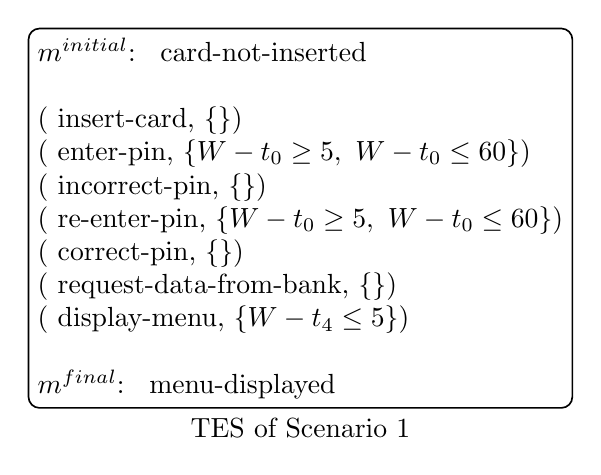
\begin{tikzpicture}[->,>=stealth']
		\tikzset{vertex/.style = {shape=rectangle,rounded corners, semithick, draw,align=left}}
		
		\node[vertex, label = below: TES of Scenario 1] (QUERY) 
		{ $m^{initial}$: { card-not-inserted} \\
			\\
			({ insert-card}, $\{\}$) \\
			({ enter-pin}, $\{W-t_0\geq 5,~W-t_0\leq 60\}$) \\
			({ incorrect-pin}, $\{\}$) \\
			({ re-enter-pin}, $\{W-t_0\geq 5,~W-t_0\leq 60\}$) \\
			({ correct-pin}, $\{\}$) \\
			({ request-data-from-bank}, $\{\}$) \\
			({ display-menu}, $\{W-t_4\leq 5\}$) \\
			\\
			$m^{final}$: { menu-displayed}
		};
		
		\end{tikzpicture}
		%\end{minipage}
		\hspace{0.5cm}
		%	\begin{minipage}{.7\textwidth}
		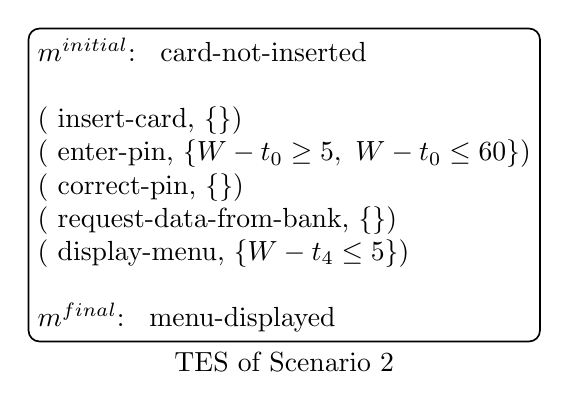
\begin{tikzpicture}[->,>=stealth']
		\tikzset{vertex/.style = {shape=rectangle,rounded corners, semithick, draw,align=left}}
		\node[vertex, label = below: TES of Scenario 2] (QUERY) 
		{ $m^{initial}$: { card-not-inserted} \\
			\\
			({ insert-card}, $\{\}$) \\
			({ enter-pin}, $\{W-t_0\geq 5,~W-t_0\leq 60\}$) \\
			({ correct-pin}, $\{\}$) \\
			({ request-data-from-bank}, $\{\}$) \\
			({ display-menu}, $\{W-t_4\leq 5\}$) \\
			\\
			$m^{final}$: { menu-displayed}
		};
		
		\end{tikzpicture}
		%	\end{minipage}
		\end{adjustbox}
		\caption{Timed Event Sequences of the ATM}
		\label{fig:TES of ATM}
	\end{figure}
\end{frame}

\begin{frame}{Constructing A Timed Automaton From Time Annotated Graph}
	 \begin{figure}[htp]
	 \centering
	 \includegraphics[width=0.9\columnwidth,height=0.8\textheight]{"ModeGraph"}
	 \caption{Mode Graph for ATM}
	 \label{fig:Mode Graph for ATM}
	 \end{figure}
\end{frame}

\begin{frame}{Constructing A Timed Automaton From Time Annotated Graph}
	\begin{columns}
		\begin{column}{0.5\textwidth}
			\begin{figure}
				\begin{adjustbox}{max totalsize={.99\textwidth}{.75\textheight},center}
					\begin{tikzpicture}[->,>=stealth',shorten >=1pt,auto,node distance=2.5cm,
					semithick]
					\tikzstyle{every state}=[shape=rectangle,draw]
					
					\node[state]       (S_0)                {$S_0$[$m_0$]};
					\node[state]         (S_1) [below of=S_0] {$S_1$[$m_1$]};
					\node[state]         (S_2) [below of=S_1] {$S_2$[$m_2$]};
					\node[state]         (S_3) [below of=S_2] {$S_3$[$m_3$]};
					\node[state]         (S_4) [below of=S_3] {$S_4$[$m_2$]};
					\node[state]         (S_5) [below of=S_4] {$S_5$[$m_4$]};
					\node[state]         (S_6) [below of=S_5] {$S_6$[$m_5$]};
					\node[state]         (S_7) [below of=S_6] {$S_7$[$m_6$]};
					
					
					\path (S_0) edge              node[left] {insert-card}                (S_1)
					(S_1) edge              node[left] {enter-pin [$W − t_0 \ge 5, W − t_0 \le 60$]}  (S_2)
					(S_2) edge        node[left] {incorrect-pin}              (S_3)
					(S_3) edge              node[left] {enter-pin [$W − t_0 \ge 5, W − t_0 \le 60$]}  (S_4)
					(S_4) edge              node[left] {correct-pin} (S_5)
					(S_5) edge        node[left] {request-data-from-bank} (S_6)
					(S_6) edge        node[left] {display-menu [$W − t_4 \le 5$]} (S_7)
					(S_2) edge [bend left]  node[right] {correct-pin} (S_5)
					;
					\end{tikzpicture}
			
				\end{adjustbox}
				\caption{Time annotated graph synthesized from two TES in Figure \ref{fig:TES of Scenario}}
				\label{fig:Time annotated graph generated by combining scenario 1 and scenario 2}
			\end{figure}			
		\end{column}
	
		\begin{column}{0.5\textwidth}
			\begin{figure}[!htb]
				\begin{adjustbox}{max totalsize={.99\textwidth}{.8\textheight},center}
					\begin{tikzpicture}[->,>=stealth',shorten >=1pt,auto,node distance=2.5cm,
					semithick]
					\tikzstyle{every state}=[draw]
					
					\node[state]       (S_0)                {$S_0$};
					\node[state]         (S_1) [below of=S_0] {$S_1$};
					\node[state]         (S_2) [below of=S_1] {$S_2$};
					\node[state]         (S_3) [below of=S_2] {$S_3$};
					\node[state]         (S_4) [below of=S_3] {$S_4$};
					\node[state]         (S_5) [below of=S_4] {$S_5$};
					\node[state]         (S_6) [below of=S_5] {$S_6$};
					\node[state]         (S_7) [below of=S_6] {$S_7$};
					
					
					\path (S_0) edge              node[left] {insert-card [$c_0 :=0$]}                (S_1)
					(S_1) edge              node[left] {enter-pin [$c_0 \ge 5, c_0 \le 60$]}  (S_2)
					(S_2) edge        node[left] {incorrect-pin}              (S_3)
					(S_3) edge              node[left] {enter-pin [$c_0 \ge 5, c_0 \le 60$]}  (S_4)
					(S_4) edge              node[left] {correct-pin} (S_5)
					(S_5) edge        node[left] {request-data-from-bank [$c_4 :=0$]} (S_6)
					(S_6) edge        node[left] {display-menu [$c_4 \le 5$]} (S_7)
					(S_2) edge [bend left]  node[right] {correct-pin} (S_5)
					;
					\end{tikzpicture}
				\end{adjustbox}
				\caption{Timed automaton constructed from time annotated graph in Figure \ref{fig:Time annotated graph generated by combining scenario 1 and scenario 2}}
				\label{fig:Timed Automaton generated by combining scenario 1 and scenario 2}
			\end{figure}	
			
		\end{column}
	\end{columns}

\end{frame}

\section{Optimal Clock Allocation of Timed Automata}

\begin{frame}{Optimal Clock Allocation of Timed Automata}
\begin{itemize}
	\item Liveness analysis
	\item Clock allocation
\end{itemize}
\end{frame}

\begin{frame}{Liveness Range Analysis}
	\begin{itemize}
		\item
		$\mathit{\textbf{clock\_ref}}$: $\mathit{clock\_ref(r)}$ is the set of clocks which are referred to in the clock constraints on $r$.
		
		\item
		$\textbf{born}$: $\Born(r)$ identifies a clock that is reset on $r$  whose value can be used on some transition	reachable from $r$.
	
		\item 
		$\textbf{active}$: $\Active(r)$ identifies clocks that are ``alive'' on $r$ (i.e., their  values may be subsequently used). Notice that $\Born(r)\subseteq \Active(r)$.
		
		\item
		$\textbf{needed}$: Maps transition $r$ to $\Active(r)\cup \mathit{clock\_ref(r)}$.
		
	\end{itemize}
\end{frame}

\begin{frame}{Liveness Range Analysis Example}
 \begin{columns}
	\begin{column}{0.4\textwidth}
		\begin{figure}
			\begin{adjustbox}{max totalsize={.99\textwidth}{.8\textheight},center}
			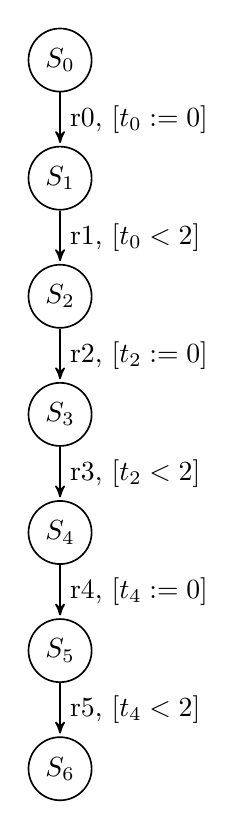
\begin{tikzpicture}[->,>=stealth',shorten >=1pt,auto,node distance=1.5cm,
			semithick]
			\tikzstyle{every state}=[draw,minimum size=1em]
			
			\node[state]         (S_0)                    {$S_0$};
			\node[state]         (S_1) [below of=S_0]     {$S_1$};
			\node[state]         (S_2) [below of=S_1]     {$S_2$};
			\node[state]         (S_3) [below of=S_2]     {$S_3$};
			\node[state]         (S_4) [below of=S_3]     {$S_4$};
			\node[state]         (S_5) [below of=S_4]     {$S_5$};
			\node[state]         (S_6) [below of=S_5]     {$S_6$};	
			
			\path (S_0) edge              node[right]  {r0, [$t_0:=0$]}  (S_1)
			(S_1) edge              node[right]  {r1, [$t_0<2$]}   (S_2)
			(S_2) edge              node[right]  {r2, [$t_2:=0$]}  (S_3)
			(S_3) edge              node[right] {r3, [$t_2<2$]}   (S_4)
			(S_4) edge              node[right] {r4, [$t_4:=0$]}  (S_5)
			(S_5) edge              node[right] {r5, [$t_4<2$]}   (S_6)
			
			;
			\end{tikzpicture}
			\end{adjustbox}
			\caption{A simple timed automaton}
			\label{fig:Simple Timed Automaton}
		\end{figure}
	\end{column}
			\begin{column}{0.5\textwidth}
			\begin{table}
				\centering
				\caption{$born$ and $active$ values}
				\label{tab:table1}
				\begin{tabular}{ccc}
					\toprule
					{ \textbf{Transition}} & { \textbf{Born}} & { \textbf{Active}} \\ \midrule
					{ $r_0$}               & { \{0\}}         & { \{0\}}           \\
					{ $r_1$}               & { $\phi$}        & { $\phi$}          \\
					{ $r_2$}               & { \{2\}}         & { \{2\}}           \\
					{ $r_3$}               & { $\phi$}        & { $\phi$}          \\
					{ $r_4$}               & { \{4\}}         & { \{4\}}           \\
					{ $r_5$}               & { $\phi$}        & { $\phi$} \\
					\bottomrule
				\end{tabular}
			\end{table}
		\end{column}
		\begin{column}{0.1\textwidth}
		\end{column}
	\end{columns}
\end{frame}

\begin{frame}

\end{frame}

\begin{frame}{ModeGraph}
	\begin{figure}
		\begin{adjustbox}{max totalsize={.99\textwidth}{.85\textheight},center}
			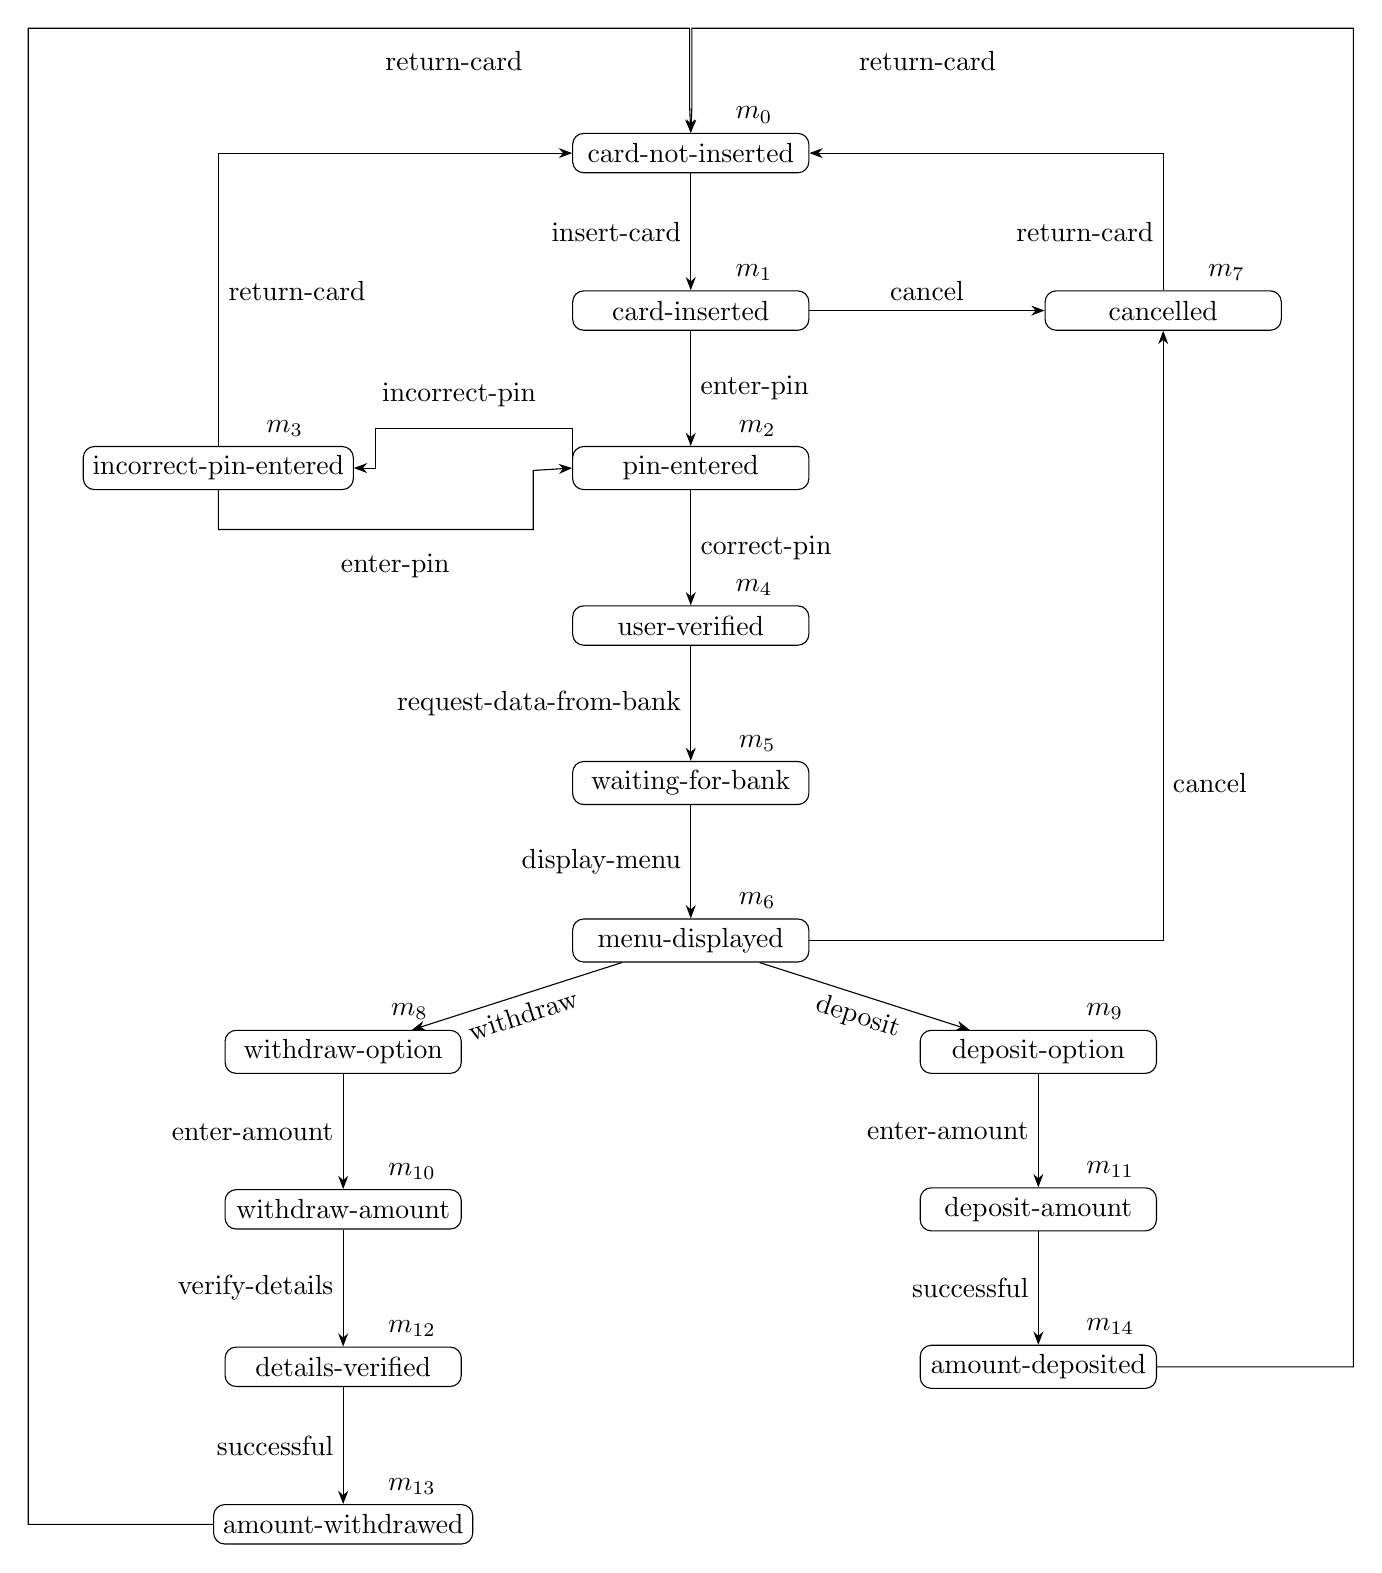
\begin{tikzpicture}[
			node distance=2cm,
			state/.style={rectangle, rounded corners, minimum width=3cm, minimum height=0.5cm,text centered, draw=black},
			process/.style={rectangle, minimum width=3cm, minimum height=0.5cm, text centered, draw=black, fill=orange!30},
			io/.style={trapezium, trapezium left angle=70, trapezium right angle=110, minimum width=3cm, minimum height=1cm, text centered, draw=black, fill=blue!30},
			decision/.style={diamond, minimum width=3cm, minimum height=1cm, text centered, draw=black, fill=green!30},
			]
			
			\node[state]       (m_0) [label={[label]30:$m_0$}]                                        {card-not-inserted};
			\node[state]         (m_1) [below of=m_0, label={[label]30:$m_1$}]                          {card-inserted};
			\node[state]         (m_2) [below of=m_1, label={[label]30:$m_2$}]                          {pin-entered};
			\node[state]         (m_3) [left of=m_2, xshift=-4cm, label={[label]30:$m_3$}]              {incorrect-pin-entered};
			\node[state]         (m_4) [below of=m_2, label={[label]30:$m_4$}]                          {user-verified};
			\node[state]         (m_5) [below of=m_4, label={[label]30:$m_5$}]                          {waiting-for-bank};
			\node[state]         (m_6) [below of=m_5, label={[label]30:$m_6$}]                          {menu-displayed};
			\node[state]         (m_7) [right of=m_1, xshift=4cm, label={[label]30:$m_7$}]              {cancelled};
			\node[state]         (m_8) [below left of=m_6, xshift=-3cm, label={[label]30:$m_8$}]        {withdraw-option};
			\node[state]         (m_9) [below right of=m_6, xshift=3cm, label={[label]30:$m_9$}]        {deposit-option};
			\node[state]         (m_10) [below of=m_8, label={[label]30:$m_{10}$}]                      {withdraw-amount};
			\node[state]         (m_11) [below of=m_9, label={[label]30:$m_{11}$}]                      {deposit-amount};
			\node[state]         (m_12) [below of=m_10, label={[label]30:$m_{12}$}]                     {details-verified};
			\node[state]         (m_13) [below of=m_12, label={[label]30:$m_{13}$}]                     {amount-withdrawed};
			\node[state]         (m_14) [below of=m_11, label={[label]30:$m_{14}$}]                     {amount-deposited};
			
			
			\draw [arrows=-Stealth] (m_0)                                                    --node[anchor=east]                                              {insert-card}        (m_1);
			\draw [arrows=-Stealth] (m_1)                                                    --node[anchor=west]                                              {enter-pin}         (m_2);
			\draw [arrows=-Stealth] (m_1)                                                    --node[anchor=south]                                             {cancel}       (m_7);
			\draw [arrows=-Stealth] (m_2.west) -- ++(0,0.5)  -- ++(-2.5,0) -- ++(0,-0.5)     --node[xshift=1.2cm,yshift=1.2cm,anchor=north,below]             {incorrect-pin}       (m_3.east);
			\draw [arrows=-Stealth] (m_3.south) -- ++(0,-0.5) -- ++(4,0) -- ++(0,0.75)       --node[xshift=-2cm,yshift=-1.5cm,anchor=south]                   {enter-pin}    (m_2.west);
			\draw [arrows=-Stealth] (m_3)                                                    |-node[xshift=1cm,yshift=-1.5cm,anchor=north,below]              {return-card} (m_0);
			\draw [arrows=-Stealth] (m_2)                                                    --node[anchor=west]                                              {correct-pin}       (m_4);
			\draw [arrows=-Stealth] (m_4)                                                    --node[anchor=east]                                              {request-data-from-bank}(m_5);
			\draw [arrows=-Stealth] (m_5)                                                    --node[anchor=east]                                              {display-menu}         (m_6);
			\draw [arrows=-Stealth] (m_6)                                                    -|node[yshift=2cm,anchor=west]                                              {cancel}       (m_7);
			\draw [arrows=-Stealth] (m_7)                                                    |-node[yshift=-1cm,anchor=east]                                              {return-card}    (m_0);
			\draw [arrows=-Stealth] (m_6)                                                    --node[anchor=north,sloped]                                      {withdraw} (m_8);
			\draw [arrows=-Stealth] (m_6)                                                    --node[anchor=north,sloped]                                      {deposit}       (m_9);
			\draw [arrows=-Stealth] (m_8)                                                    --node[anchor=east]                                              {enter-amount}        (m_10);
			\draw [arrows=-Stealth] (m_10)                                                   --node[anchor=east]                                              {verify-details}   (m_12);
			\draw [arrows=-Stealth] (m_12)                                                   --node[anchor=east]                                              {successful}       (m_13);
			\draw [arrows=-Stealth] (m_13) -- ++(-4,0) -- ++(0,19) -- ++(8.4,0) -- ++(0,-1)              --node[xshift=-3cm,yshift=0.5cm,anchor=south]                     {return-card}    (m_0.north);
			\draw [arrows=-Stealth] (m_9)                                                    --node[anchor=east]                                              {enter-amount} (m_11);
			\draw [arrows=-Stealth] (m_11)                                                   --node[anchor=east]                                              {successful}       (m_14);
			\draw [arrows=-Stealth] (m_14) -- ++(4,0) -- ++(0,17) -- ++(-8.4,0) -- ++(0,-1)               -- node[xshift=3cm,yshift=0.5cm,anchor=south]                                            {return-card} (m_0.north);
			
			\end{tikzpicture}
		\end{adjustbox}
			\caption{Mode graph of the ATM}
			\label{fig:Mode graph of the ATM}
	\end{figure}
\end{frame}

\section{Case Studies}

\begin{frame}{Automated Teller Machine (ATM)}
Explain original scenario
\end{frame}

\begin{frame}{Automated Teller Machine (ATM)}
	\begin{figure}
		\begin{adjustbox}{max totalsize={.99\textwidth}{.85\textheight},center}
		%	\begin{minipage}{.7\textwidth}
			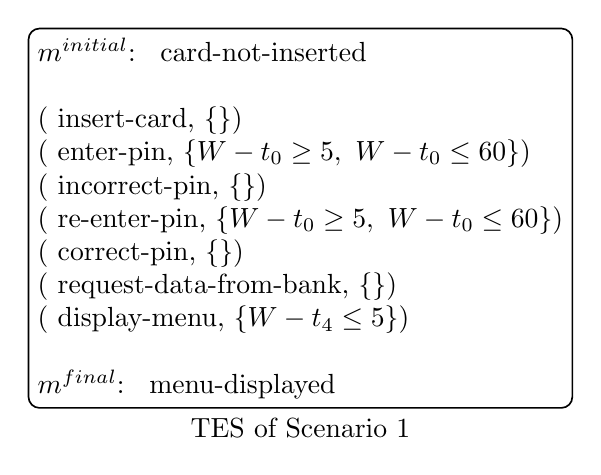
\begin{tikzpicture}[->,>=stealth']
			\tikzset{vertex/.style = {shape=rectangle,rounded corners, semithick, draw,align=left}}
			
			\node[vertex, label = below: TES of Scenario 1] (QUERY) 
			{ $m^{initial}$: { card-not-inserted} \\
				\\
				({ insert-card}, $\{\}$) \\
				({ enter-pin}, $\{W-t_0\geq 5,~W-t_0\leq 60\}$) \\
				({ incorrect-pin}, $\{\}$) \\
				({ re-enter-pin}, $\{W-t_0\geq 5,~W-t_0\leq 60\}$) \\
				({ correct-pin}, $\{\}$) \\
				({ request-data-from-bank}, $\{\}$) \\
				({ display-menu}, $\{W-t_4\leq 5\}$) \\
				\\
				$m^{final}$: { menu-displayed}
			};
			
			\end{tikzpicture}
		%\end{minipage}
		\hspace{0.5cm}
	%	\begin{minipage}{.7\textwidth}
			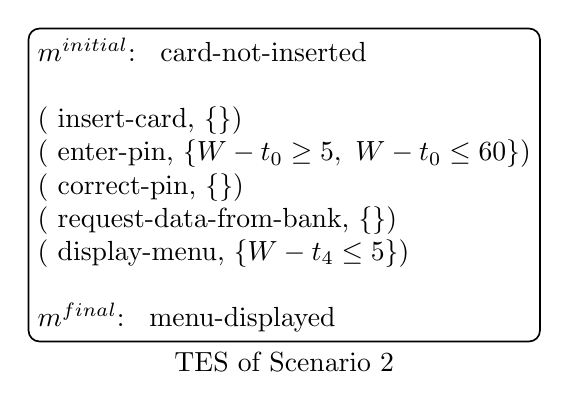
\begin{tikzpicture}[->,>=stealth']
			\tikzset{vertex/.style = {shape=rectangle,rounded corners, semithick, draw,align=left}}
			\node[vertex, label = below: TES of Scenario 2] (QUERY) 
			{ $m^{initial}$: { card-not-inserted} \\
				\\
				({ insert-card}, $\{\}$) \\
				({ enter-pin}, $\{W-t_0\geq 5,~W-t_0\leq 60\}$) \\
				({ correct-pin}, $\{\}$) \\
				({ request-data-from-bank}, $\{\}$) \\
				({ display-menu}, $\{W-t_4\leq 5\}$) \\
				\\
				$m^{final}$: { menu-displayed}
			};
			
			\end{tikzpicture}
	%	\end{minipage}
		\end{adjustbox}
		\caption{Timed Event Sequences of the ATM}
		\label{fig:Timed Event Sequences of ATM}
		
	\end{figure}
\end{frame}

\begin{frame}{Automated Teller Machine (ATM)}
	\begin{figure}
		\begin{adjustbox}{max totalsize={.99\textwidth}{.85\textheight},center}
		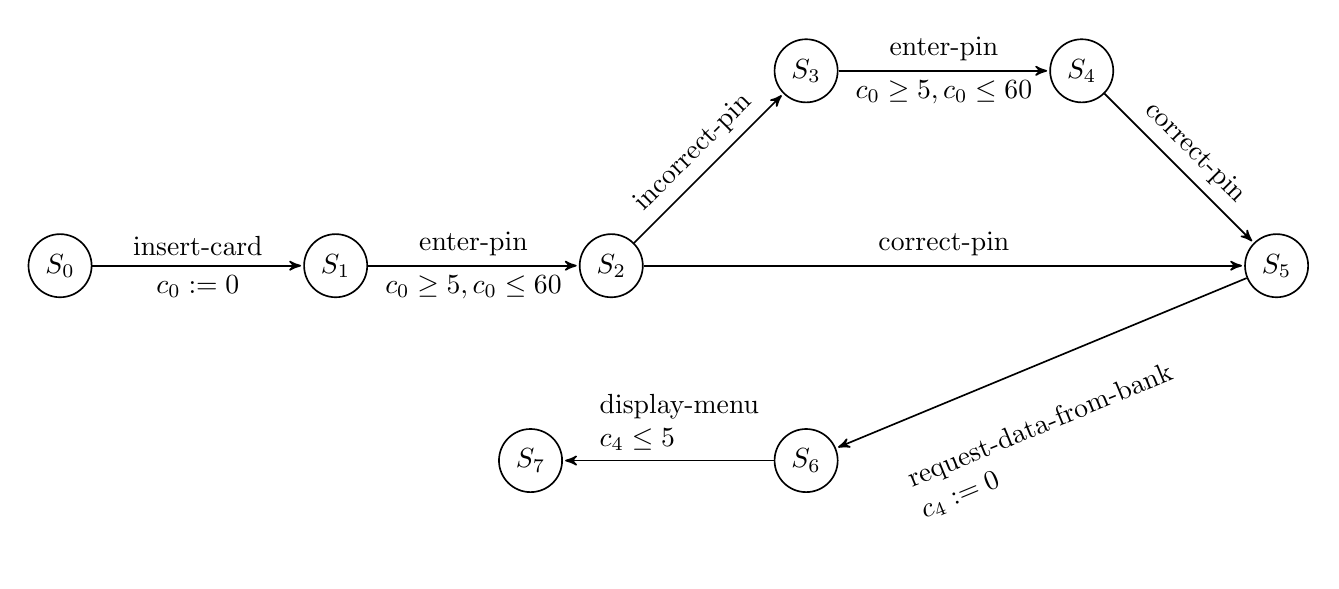
\begin{tikzpicture}[->,>=stealth',shorten >=0.8pt,auto,node distance=3.5cm,
		semithick]
		\tikzstyle{every state}=[draw,minimum size=1em]
		
		\node[state]         (S_0)              {$S_0$};
		\node[state]         (S_1) [right of=S_0] {$S_1$};
		\node[state]         (S_2) [right of=S_1] {$S_2$};
		\node[state]         (S_3) [above right of=S_2] {$S_3$};
		\node[state]         (S_4) [right of=S_3] {$S_4$};
		\node[state]         (S_5) [below right of=S_4] {$S_5$};
		\node[state]         (S_6) [below right of=S_2] {$S_6$};
		\node[state]         (S_7) [left of=S_6] {$S_7$}; 
		
		\path (S_0) edge                node[anchor=south, above]             {insert-card}           
		node[anchor=south, below]             {$c_0 := 0$}            (S_1)
		(S_1) edge                node[anchor=south, above]             {enter-pin} 
		node[anchor=north, below]             {$c_0\ge5,c_0\le60$}    (S_2)
		(S_2) edge                node[anchor=south, above,sloped]      {incorrect-pin}         (S_3)
		(S_3) edge                node[anchor=south, above]             {enter-pin} 
		node[anchor=north, below]             {$c_0\ge5,c_0\le60$}    (S_4)
		(S_4) edge                node[anchor=south, above,sloped]      {correct-pin}           (S_5)
		(S_2) edge                node[above]                           {correct-pin}           (S_5)
		(S_5) edge                node[anchor=north, below,sloped,text width=6cm]      {
			\centering
			\begin{itemize}
			\item[] request-data-from-bank\\$c_4 := 0$ 
			\end{itemize}
		}                       (S_6)
		(S_6) edge                node[anchor=south, above,text width=3.5cm] {
			\begin{itemize}
			\item[] display-menu\\$c_4\le5$
			\end{itemize}
		}                       (S_7)
		;
		\end{tikzpicture}
		\end{adjustbox}
		\caption{Timed automaton synthesized from Scenario 1 and Scenario 2}
		\label{fig:timedAutomaton}
	\end{figure}
\end{frame}

\begin{frame}{Automated Teller Machine (ATM)}
Explain extended scenario
\end{frame}

\begin{frame}{Automated Teller Machine (ATM)}
\begin{figure}
	\begin{adjustbox}{max totalsize={.99\textwidth}{.85\textheight},center}
		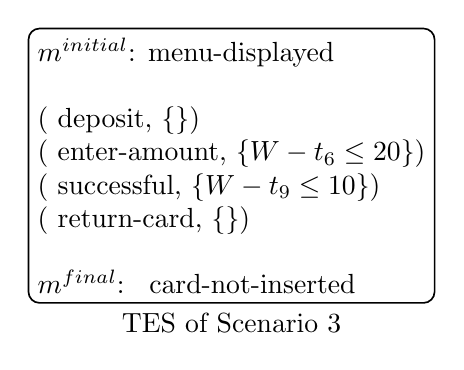
\begin{tikzpicture}[->,>=stealth']
		\tikzset{vertex/.style = {shape=rectangle,rounded corners, semithick, draw,align=left}}
		\node[vertex, label = below: TES of Scenario 3] (QUERY) 
		{ $m^{initial}$: {menu-displayed} \\
			\\
			({ deposit}, $\{\}$) \\
			({ enter-amount}, $\{W-t_6\leq 20\}$) \\
			({ successful}, $\{W-t_{9}\leq 10\}$) \\
			({ return-card}, $\{\}$) \\
			\\
			$m^{final}$: { card-not-inserted}
		};
		
		\end{tikzpicture}
	
		\hspace{0.5cm}
	
		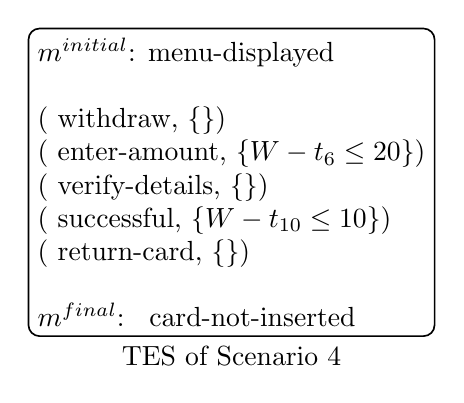
\begin{tikzpicture}[->,>=stealth']
		\tikzset{vertex/.style = {shape=rectangle,rounded corners, semithick, draw,align=left}}
		\node[vertex, label = below: TES of Scenario 4] (QUERY) 
		{ $m^{initial}$: {menu-displayed} \\
			\\
			({ withdraw}, $\{\}$) \\
			({ enter-amount}, $\{W-t_6\leq 20\}$) \\
			({ verify-details}, $\{\}$) \\
			({ successful}, $\{W-t_{10}\leq 10\}$) \\
			({ return-card}, $\{\}$) \\
			\\
			$m^{final}$: { card-not-inserted}
		};
		
		\end{tikzpicture}
		\end{adjustbox}
		\caption{Timed Event Sequences of the ATM with withdraw and deposit option}
		\label{fig:Timed Event Sequences of ATM with withdraw and deposit option}
	\end{figure}

\end{frame}

\begin{frame}{Automated Teller Machine (ATM)}
	\begin{figure}
		\begin{adjustbox}{max totalsize={.99\textwidth}{.85\textheight},center}			
			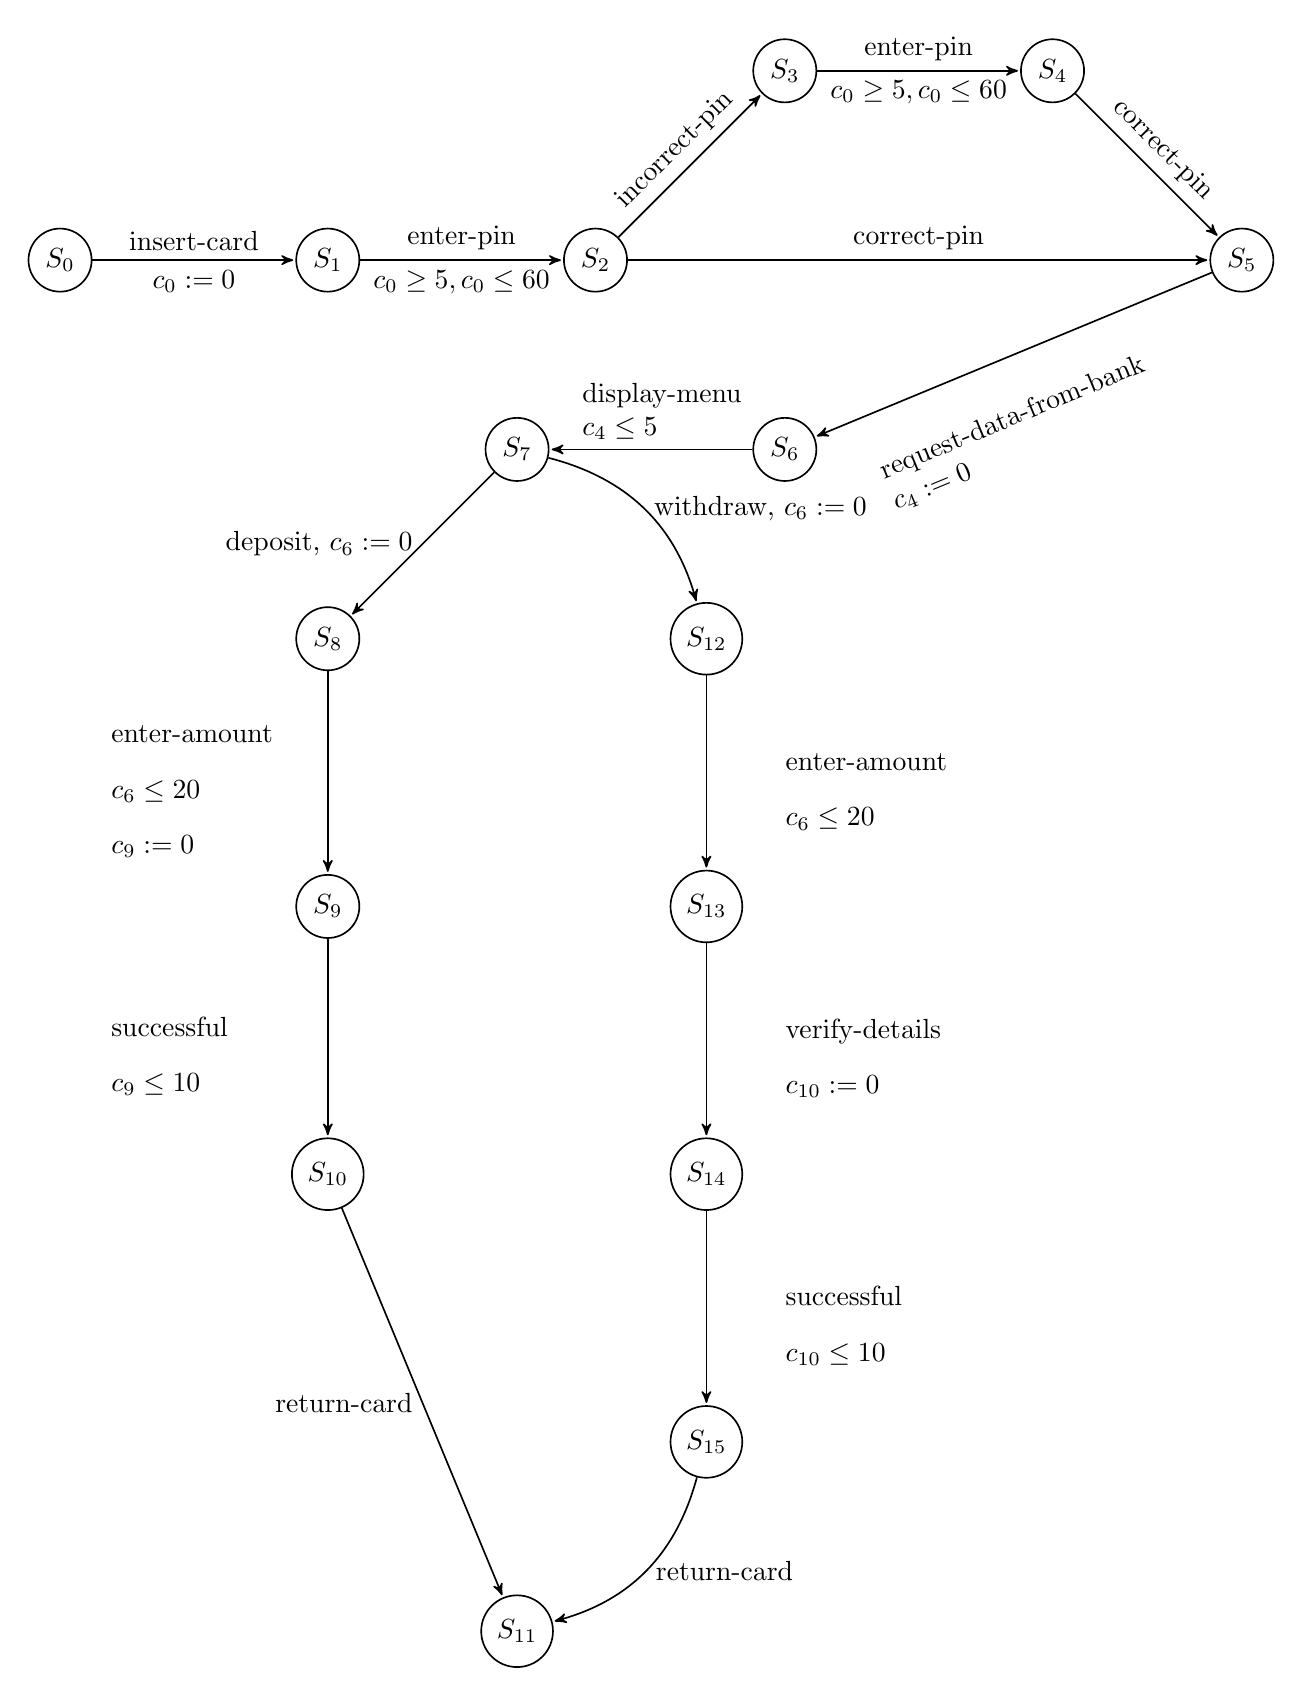
\begin{tikzpicture}[->,>=stealth',shorten >=0.8pt,auto,node distance=3.4cm,
			semithick]
			\tikzstyle{every state}=[draw,minimum size=1em]
			
			\node[state]         (S_0)              {$S_0$};
			\node[state]         (S_1) [right of=S_0] {$S_1$};
			\node[state]         (S_2) [right of=S_1] {$S_2$};
			\node[state]         (S_3) [above right of=S_2] {$S_3$};
			\node[state]         (S_4) [right of=S_3] {$S_4$};
			\node[state]         (S_5) [below right of=S_4] {$S_5$};
			\node[state]         (S_6) [below right of=S_2] {$S_6$};
			\node[state]         (S_7) [left of=S_6] {$S_7$};
			\node[state]         (S_8) [below left of=S_7] {$S_8$};
			
			\node[state]         (S_9) [below of=S_8] {$S_9$};
			\node[state]         (S_10) [below of=S_9] {$S_{10}$};
			
			\node[state]         (S_12) [below right of=S_7] {$S_{12}$};
			\node[state]         (S_13) [below of=S_12] {$S_{13}$};
			\node[state]         (S_14) [below of=S_13] {$S_{14}$};
			\node[state]         (S_15) [below of=S_14] {$S_{15}$};
			\node[state]         (S_11) [below left of=S_15] {$S_{11}$};
			
						
			\path (S_0) edge                node[anchor=south, above]             {insert-card}           
			node[anchor=south, below]             {$c_0 := 0$}            (S_1)
			(S_1) edge                node[anchor=south, above]             {enter-pin} 
			node[anchor=north, below]             {$c_0\ge5,c_0\le60$}    (S_2)
			(S_2) edge                node[anchor=south, above,sloped]      {incorrect-pin}         (S_3)
			(S_3) edge                node[anchor=south, above]             {enter-pin} 
			node[anchor=north, below]             {$c_0\ge5,c_0\le60$}    (S_4)
			(S_4) edge                node[anchor=south, above,sloped]      {correct-pin}           (S_5)
			(S_2) edge                node[above]                           {correct-pin}           (S_5)
			(S_5) edge                node[anchor=north, below,sloped,text width=6cm]      {
				\centering
				\begin{itemize}
				\item[] request-data-from-bank\\$c_4 := 0$ 
				\end{itemize}
			}                       (S_6)
			(S_6) edge                node[anchor=south, above,text width=3.5cm] 
			{ 
				\begin{itemize}
				\item[] display-menu\\$c_4\le5$
				\end{itemize}
			}                       (S_7)
			(S_7) edge                node[left]                            {deposit, $c_6:=0$}               (S_8)
			
			(S_8) edge                node[anchor=right, left,text width=3.5cm] 
			{ 
				\begin{itemize}
				\item[] enter-amount
				\item[] $c_6\le20$
				\item[] $c_9:=0$
				\end{itemize}
			}                        (S_9)
			(S_9) edge                node[anchor=right, left,text width=3.5cm] 
			{ 
				\begin{itemize}
				\item[] successful
				\item[] $c_{9}\le10$
				\end{itemize}
			}                       (S_10)
			(S_10) edge               node[left]                            {return-card}           (S_11)
			
			(S_7) edge   [bend left]  node[right]                           {withdraw, $c_6:=0$}              (S_12)
			(S_12) edge               node[anchor=left, right,text width=3.5cm] 
			{ 
				\begin{itemize}
				\item[] enter-amount
				\item[] $c_6\le20$
				\end{itemize}
			}                       (S_13)
			(S_13) edge               node[anchor=left, right,text width=3.5cm] 
			{ 
				\begin{itemize}
				\item[] verify-details
				\item[] $c_{10}:= 0$
				\end{itemize}
			}                       (S_14)
			(S_14) edge               node[anchor=left, right,text width=3.5cm] 
			{ 
				\begin{itemize}
				\item[] successful
				\item[] $c_{10}\le10$
				\end{itemize}
			}                       (S_15)
			(S_15) edge  [bend left]  node[right]                           {return-card}           (S_11)
			;
			\end{tikzpicture}
		\end{adjustbox}
		\caption{The synthesized timed automaton of the ATM}
		\label{fig:Synthesized ATM TA}
	\end{figure}
\end{frame}


\begin{frame}{Light Control System}
	\begin{figure}[!ht]
		\begin{center}
%			\begin{minipage}{0.8\textwidth}
				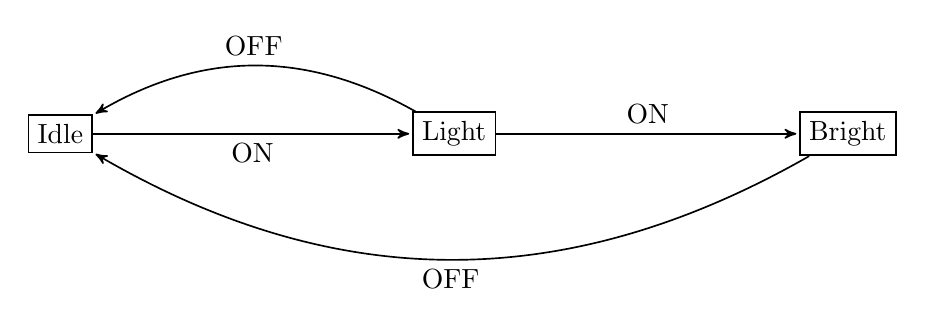
\begin{tikzpicture}[->,>=stealth',shorten >=1pt,auto,node distance=5cm,
				semithick]
				\tikzstyle{every state}=[shape=rectangle,draw,minimum size=1em]
				
				\node[state]       (Idle)                    {Idle};
				\node[state]       (Light)  [right of=Idle]     {Light};
				\node[state]       (Bright) [right of=Light]     {Bright};
				
				\path (Idle) edge                   node[below]  {ON}  (Light)
				(Light) edge    [bend right]  node[above]  {OFF}  (Idle)
				(Light) edge                  node[above]  {ON}  (Bright)
				(Bright) edge   [bend left]   node[below]  {OFF}  (Idle)    
				;
				\end{tikzpicture}
%			\end{minipage}
		\end{center}
		\caption{Mode graph of the Light Control System}
		\label{fig:MG_Light Control System}
		\vspace{0.1cm}
	\end{figure}
\end{frame}

\begin{frame}{Light Control System}
		\begin{figure}
			\begin{adjustbox}{max totalsize={.99\textwidth}{.85\textheight},center}
	
%			\begin{minipage}[b]{.25\textwidth}
				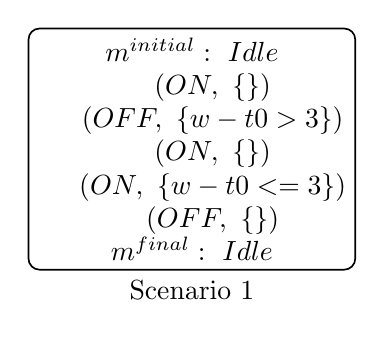
\begin{tikzpicture}[->,>=stealth']
				\tikzset{vertex/.style = {shape=rectangle,rounded corners, semithick, draw,align=center}}
				\node[vertex, label = below: Scenario 1] (QUERY) 
				{$m^{initial}:~Idle$ \\                                
					\indent    ($ON,~\{\}$) \\
					\indent    ($OFF, ~\{w-t0 > 3\}$) \\
					\indent    ($ON,~\{\}$) \\
					\indent    ($ON, ~\{w-t0 <= 3\}$) \\
					\indent    ($OFF,~\{\}$) \\                
					$m^{final}:~Idle$};
				
				\end{tikzpicture}
%			\end{minipage}
			\hspace{0.5cm}
%			\begin{minipage}[b]{.25\textwidth}
				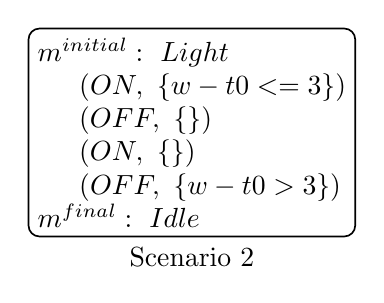
\begin{tikzpicture}[->,>=stealth']
				\tikzset{vertex/.style = {shape=rectangle,rounded corners, semithick, draw,align=left}}
				\node[vertex, label = below: Scenario 2] (QUERY) 
				{$m^{initial}:~Light$ \\
					
					\indent    ($ON,~\{w-t0 <= 3\}$) \\
					\indent    ($OFF,~\{\}$) \\
					\indent    ($ON,~\{\}$) \\
					\indent    ($OFF,~\{w-t0 > 3\}$) \\
					
					$m^{final}:~Idle$};
				
				\end{tikzpicture}
%			\end{minipage}
			\hspace{0.5cm}
%			\begin{minipage}[b]{.25\textwidth}
				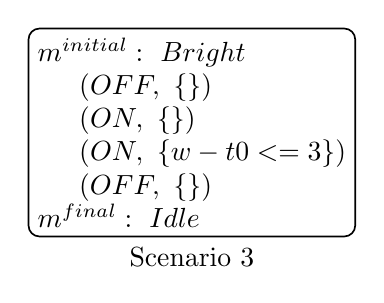
\begin{tikzpicture}[->,>=stealth']
				\tikzset{vertex/.style = {shape=rectangle,rounded corners, semithick, draw,align=left}}
				\node[vertex, label = below: Scenario 3] (QUERY) 
				{$m^{initial}:~Bright$ \\
					
					\indent    ($OFF,~\{\}$) \\
					\indent    ($ON,~\{\}$) \\
					\indent    ($ON,~\{w-t0 <= 3\}$) \\
					\indent    ($OFF,~\{\}$) \\
					
					$m^{final}:~Idle$};
				
				\end{tikzpicture}
%			\end{minipage}
		
		\end{adjustbox}
		\caption{Timed Event Sequences of the Light Control System}
		\label{fig:Timed Event Sequences of Light Control System}
	\end{figure}
\end{frame}

\begin{frame}{Light Control System}
	\begin{figure}
		\begin{adjustbox}{max totalsize={.99\textwidth}{.8\textheight},center}
			\begin{tikzpicture}[->,>=stealth',shorten >=1pt,auto,node distance=2.3cm,
			semithick]
			\tikzstyle{every state}=[draw,minimum size=1.65cm]
			
			\node[state]         (S_0) [yshift=-1.5cm]                   {$Idle$};
			\node[state]         (S_1) [below of=S_0,yshift=-1cm]     {$Light$};
			\node[state]         (S_2) [below of=S_1,yshift=-1cm]     {$Idle$};
			\node[state]         (S_3) [below of=S_2,yshift=-1cm]     {$Light$};
			\node[state]         (S_4) [below of=S_3,yshift=-1cm]   {$Bright$};
			\node[state]         (S_5) [right of=S_4,xshift=1cm]    {$Idle$};
			\node[state]         (S_6) [right of=S_5,xshift=1.6cm]    {$Light$};
			\node[state]         (S_7) [right of=S_6,xshift=1.6cm]    {$Idle$};
			\node[state]         (S_8) [above right of=S_6,xshift=1cm,yshift=1cm]    {$Bright$};
			
			\path (S_0) edge              node[right]  {ON [$c_0 := 0$]}  (S_1)
			(S_1) edge              node[right]  {OFF [$c_0 > 3$]}  (S_2)
			(S_2) edge              node[right]  {ON [$c_0 := 0$]}  (S_3)
			(S_1) edge [bend right] node[left]   {ON [$c_0 <= 3$]}  (S_4)
			(S_3) edge              node[right]  {ON [$c_0 <= 3$]}  (S_4)
			(S_4) edge              node[below]  {OFF}  (S_5)
			(S_5) edge              node[below]  {ON [$c_0 := 0$]}  (S_6)
			(S_6) edge              node[below]  {OFF [$c_0 > 3$]}  (S_7)
			(S_6) edge [bend left]  node[left]   {ON [$c_0 <= 3$]}  (S_8)
			(S_8) edge [bend left]  node[right]  {OFF}  (S_7)
			
			;
			\end{tikzpicture}
		\end{adjustbox}
	
		\caption{Timed automaton of the Light Control System}
		\label{fig:TA_Ligt Control System}
	\end{figure}
\end{frame}

\begin{frame}{Traffic Light}
	\begin{figure}
		\begin{adjustbox}{max totalsize={.99\textwidth}{.8\textheight},center}
		
		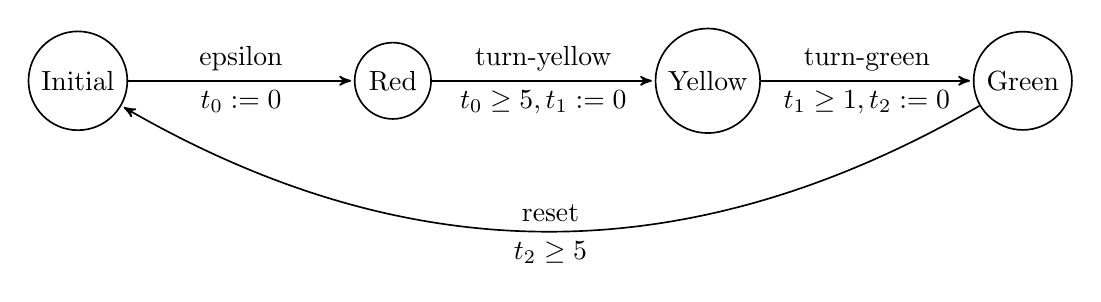
\begin{tikzpicture}[->,>=stealth',shorten >=1pt,auto,node distance=4cm,
		semithick]
		\tikzstyle{every state}=[draw,minimum size=1em]
		
		\node[state]       (Initial)                        {Initial};
		\node[state]       (Red)      [right of=Initial]    {Red};
		\node[state]       (Yellow)   [right of=Red]        {Yellow};
		\node[state]       (Green)    [right of=Yellow]      {Green};
		
		
		\path (Initial)   edge          node[anchor=south, above] {epsilon} 
		node[anchor=north, below] {$t_0:=0$}       (Red)
		(Red)       edge                 node[anchor=south, above] {turn-yellow}
		node[anchor=north, below] {$t_0\ge5,t_1:=0$}     (Yellow)
		(Yellow)    edge                 node[anchor=south, above] {turn-green} 
		node[anchor=north, below] {$t_1\ge1,t_2:=0$}     (Green)
		(Green)     edge   [bend left]   node[anchor=south, above] {reset} 
		node[anchor=north, below] {$t_2\ge5$}           (Initial)   
		;
		\end{tikzpicture}
		\end{adjustbox}
		\caption{Timed automaton of the Traffic Light}
		\label{fig:TrafficLight}		
	\end{figure}
\end{frame}

\begin{frame}{Traffic Light}
	\begin{figure}
		\begin{adjustbox}{max totalsize={.99\textwidth}{.8\textheight},center}		
	
		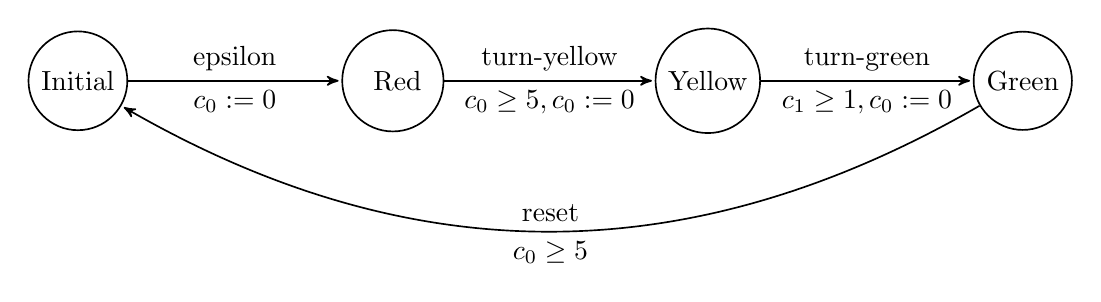
\begin{tikzpicture}[->,>=stealth',shorten >=1pt,auto,node distance=4cm,
		semithick]
		\tikzstyle{every state}=[draw,minimum size=1em]
		
		\node[state]       (Initial)                        {Initial};
		\node[state]       (Red)      [right of=Initial]    {~~Red~~};
		\node[state]       (Yellow)   [right of=Red]        {Yellow};
		\node[state]       (Green)    [right of=Yellow]      {Green};
		
		
		\path (Initial)   edge          node[anchor=south, above] {epsilon} 
		node[anchor=north, below] {$c_0:=0$}       (Red)
		(Red)       edge                 node[anchor=south, above] {turn-yellow}
		node[anchor=north, below] {$c_0\ge5,c_0:=0$}     (Yellow)
		(Yellow)    edge                 node[anchor=south, above] {turn-green} 
		node[anchor=north, below] {$c_1\ge1,c_0:=0$}     (Green)
		(Green)     edge   [bend left]   node[anchor=south, above] {reset} 
		node[anchor=north, below] {$c_0\ge5$}           (Initial)   
		;
		\end{tikzpicture}
	
		\end{adjustbox}
		\caption{The optimally allocated timed automaton of the Traffic Light}
		\label{fig:OptimalTrafficLight}
	\end{figure}
\end{frame}

\begin{frame}{CSMA/CD Protocol}
	\begin{figure}
		\begin{adjustbox}{max totalsize={.99\textwidth}{.8\textheight},center}	
			\begin{tikzpicture}[->,>=stealth',shorten >=1pt,auto,node distance=8cm,
			semithick]
			\tikzstyle{every state}=[draw,minimum size=2cm]
			
			\node[state]         (init)                    {$init$};
			\node[state]         (send) [right of=init]  {$send$};
			\node[state]         (cd_1) [below right of=send]  {$cd_1$};
			\node[state]         (transm) [left of=cd_1] {$transm$};
			\node[state]         (cd_2) [below of=transm]  {$cd_2$};
			
			
			\path (init) edge                   node[below] {r1  [$x_0:=0$]}  (send)
			(init) edge   [bend left]     node[above] {r11 [$x_0:=0$]}  (send)
			(init) edge   [loop above]    node[]      {r10}  (init)
			(send) edge   [bend right]    node[sloped,anchor=center,below,text width=4cm]  {r2  [$x_0=0,x_1:=0$]}  (cd_1)
			(send) edge                   node[sloped,anchor=center,below,text width=4cm]  {r3  [$x_0=0,x_1:=0$]}  (cd_1)
			(send) edge                   node[sloped,anchor=center,above,text width=4cm]  {r5  [$x_0=0,x_1:=0$]}  (transm)
			(cd_1) edge   [bend right]    node[sloped,anchor=center,above,text width=3cm] {r4  [$x_1<=2\sigma$]}  (send)
			(cd_1) edge   [loop below]    node[]      {r9}  (cd_1)
			(transm) edge                 node[sloped,anchor=center,above,text width=2cm]  {r6  [$x_1=\lambda$]}  (init)
			(transm) edge [bend left]     node[right]  {r7  [$x_1<=\lambda,x_3:=0$]}  (cd_2)
			(cd_2) edge   [bend  left]    node[sloped,anchor=center,above,text width=3cm]  {r8  [$x_3<=2\lambda$]}  (init)
			
			;
			\end{tikzpicture}
		\end{adjustbox}
		\caption{The timed automaton for the sender in CSMA/CD protocol}
		\label{fig:CSMA/CD}
	\end{figure}
\end{frame}


\begin{frame}{CSMA/CD Protocol}
	\begin{figure}
		\begin{adjustbox}{max totalsize={.99\textwidth}{.8\textheight},center}	

		\begin{tikzpicture}[->,>=stealth',shorten >=1pt,auto,node distance=8cm,
		semithick]
		\tikzstyle{every state}=[draw,minimum size=2cm]
		
		\node[state]         (init)                    {$init$};
		\node[state]         (send) [right of=init]  {$send$};
		\node[state]         (cd_1) [below right of=send]  {$cd_1$};
		\node[state]         (transm) [left of=cd_1] {$transm$};
		\node[state]         (cd_2) [below of=transm]  {$cd_2$};
		
		
		\path (init) edge                   node[below]                                      {r1  [$c_1:=0$]}  (send)
		(init) edge   [bend left]     node[above]                                      {r11 [$c_1:=0$]}  (send)
		(init) edge   [loop above]    node[]                                           {r10}             (init)
		(send) edge   [bend right]    node[sloped,anchor=center,below,text width=4cm]  {r2  [$c_1=0,c_2:=0$]}  (cd_1)
		(send) edge                   node[sloped,anchor=center,below,text width=4cm]  {r3  [$c_1=0,c_2:=0$]}  (cd_1)
		(send) edge                   node[sloped,anchor=center,above,text width=4cm]  {r5  [$c_1=0,c_2:=0$]}  (transm)
		(cd_1) edge   [bend right]    node[sloped,anchor=center,above,text width=3cm]  {r4  [$c_2<=2\sigma$]}  (send)
		(cd_1) edge   [loop below]    node[]                                           {r9}                    (cd_1)
		(transm) edge                 node[sloped,anchor=center,above,text width=2cm]  {r6  [$c_1=\lambda$]}  (init)
		(transm) edge [bend left]     node[right]                                      {r7  [$c_1<=\lambda,c_1:=0$]}  (cd_2)
		(cd_2) edge   [bend  left]    node[sloped,anchor=center,above,text width=3cm]  {r8  [$c_1<=2\lambda$]}  (init)
		
		;
		\end{tikzpicture}
		\end{adjustbox}
		\caption{The optimally allocated timed automaton for the sender in CSMA/CD protocol}
		\label{fig:OptimalCSMA/CD}
	\end{figure}
\end{frame}

\section{Conclusion}

\begin{frame}{Conclusion}
	conclude here
	\cite{FromScenariosToTimedAutomata-2016}
	\cite{OptimalClockAllocationTA}
\end{frame}

\begin{frame}[standout]
	Questions?
\end{frame}


\begin{frame}[allowframebreaks]{References}
	\bibliography{ResearchPPT}
	\bibliographystyle{abbrv}
\end{frame}

\end{document}